\chapterimage{chapter_bg.pdf} % Chapter heading image
%\chapterspaceabove{6.75cm} % Whitespace from the top of the page to the chapter title on chapter pages
%\chapterspacebelow{7.25cm} % Amount of vertical whitespace from the top margin to the start of the text on chapter pages

\chapter{Introdução}

O mundo tem hoje mais de 4.7 bilhões de usuários de internet, sendo que cada usuário padrão passa cerca de 6 horas e meia por dia navegando. Conquistar um pouco da atenção desse usuário, seja através de um site ou de uma página em rede social, deixou de ser algo opcional. 

Não é à toa que existem mais 1.8 bilhão de sites na web atualmente. Consequentemente, nunca houve tanta demanda por profissionais capazes de criar e administrar sites. Se você quer aproveitar essa oportunidade aprendendo a criar e a publicar sites, você está no lugar certo. Vale ressaltar que este material é totalmente voltado para iniciantes, isto é, para quem realmente não sabe nada sobre criação de sites. 

\section{O Funcionamento de um Site}

Nesta seção, eu vou explicar os princípios básicos de funcionamento de um site, para que, antes de começar a codificar, você entenda como as coisas funcionam nos bastidores. Essa compreensão é imprescindível para que você consiga criar sites de qualidade de jeito certo. 

Um site é composto por uma ou mais páginas de hipertexto. Diferentemente de um texto comum, uma página de hipertexto corresponde a uma página que pode conter textos, imagens e elementos multimídia de forma combinada para comunicar alguma ideia. Mas o principal diferencial de uma página de hipertexto é que ela pode conter ligações com outras páginas, de forma que o leitor possa navegar para essas outras páginas através dessas ligações, que são chamadas de hiperlinks, ou simplesmente \textit{links}. A figura \ref{fig:siteslinked} apresenta exemplos fictíticos de sites que possuem hiperlinks conectando-os.

\begin{figure}[htbp!]
    \centering
    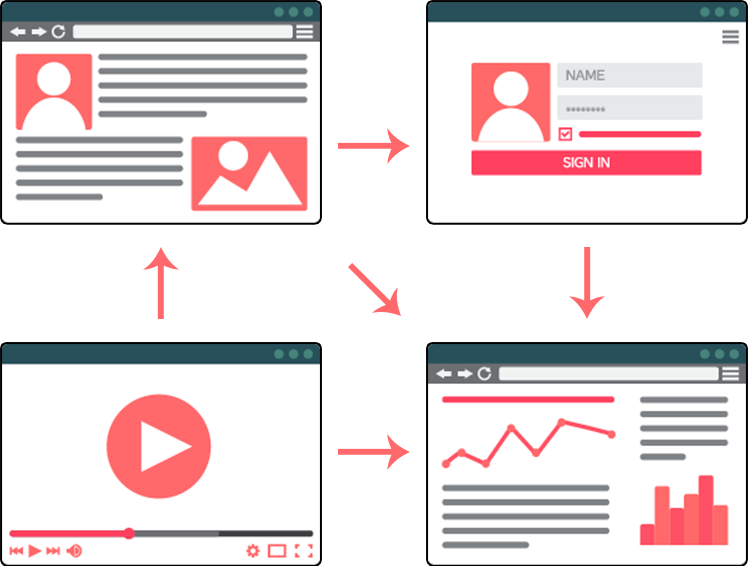
\includegraphics[width=0.6\textwidth]{Images/chapter01/sites_linkados.png}
    \caption{Sites conectados através de hiperlinks.}
    \label{fig:siteslinked}
\end{figure}

Nos bastidores, para que o navegador consiga exibir o conteúdo da forma como você está acostumado a ver quando navega pela web, um texto contendo um conjunto de instruções deve indicar ao navegador \textbf{quais} elementos devem ser exibidos e \textbf{como} esses elementos devem ser exibidos. Essas instruções interpretadas pelo navegador são chamadas de \textbf{códigos}, que nada mais são do que textos escritos em um padrão que chamamos de \textbf{linguagem}. Toda página de um site, basicamente, é uma combinação de códigos escritos em três linguagens diferentes: HTML, CSS e Javascript, como mostra a figura \ref{fig:sitescodigo}.

\begin{figure}[htbp!]
    \centering
    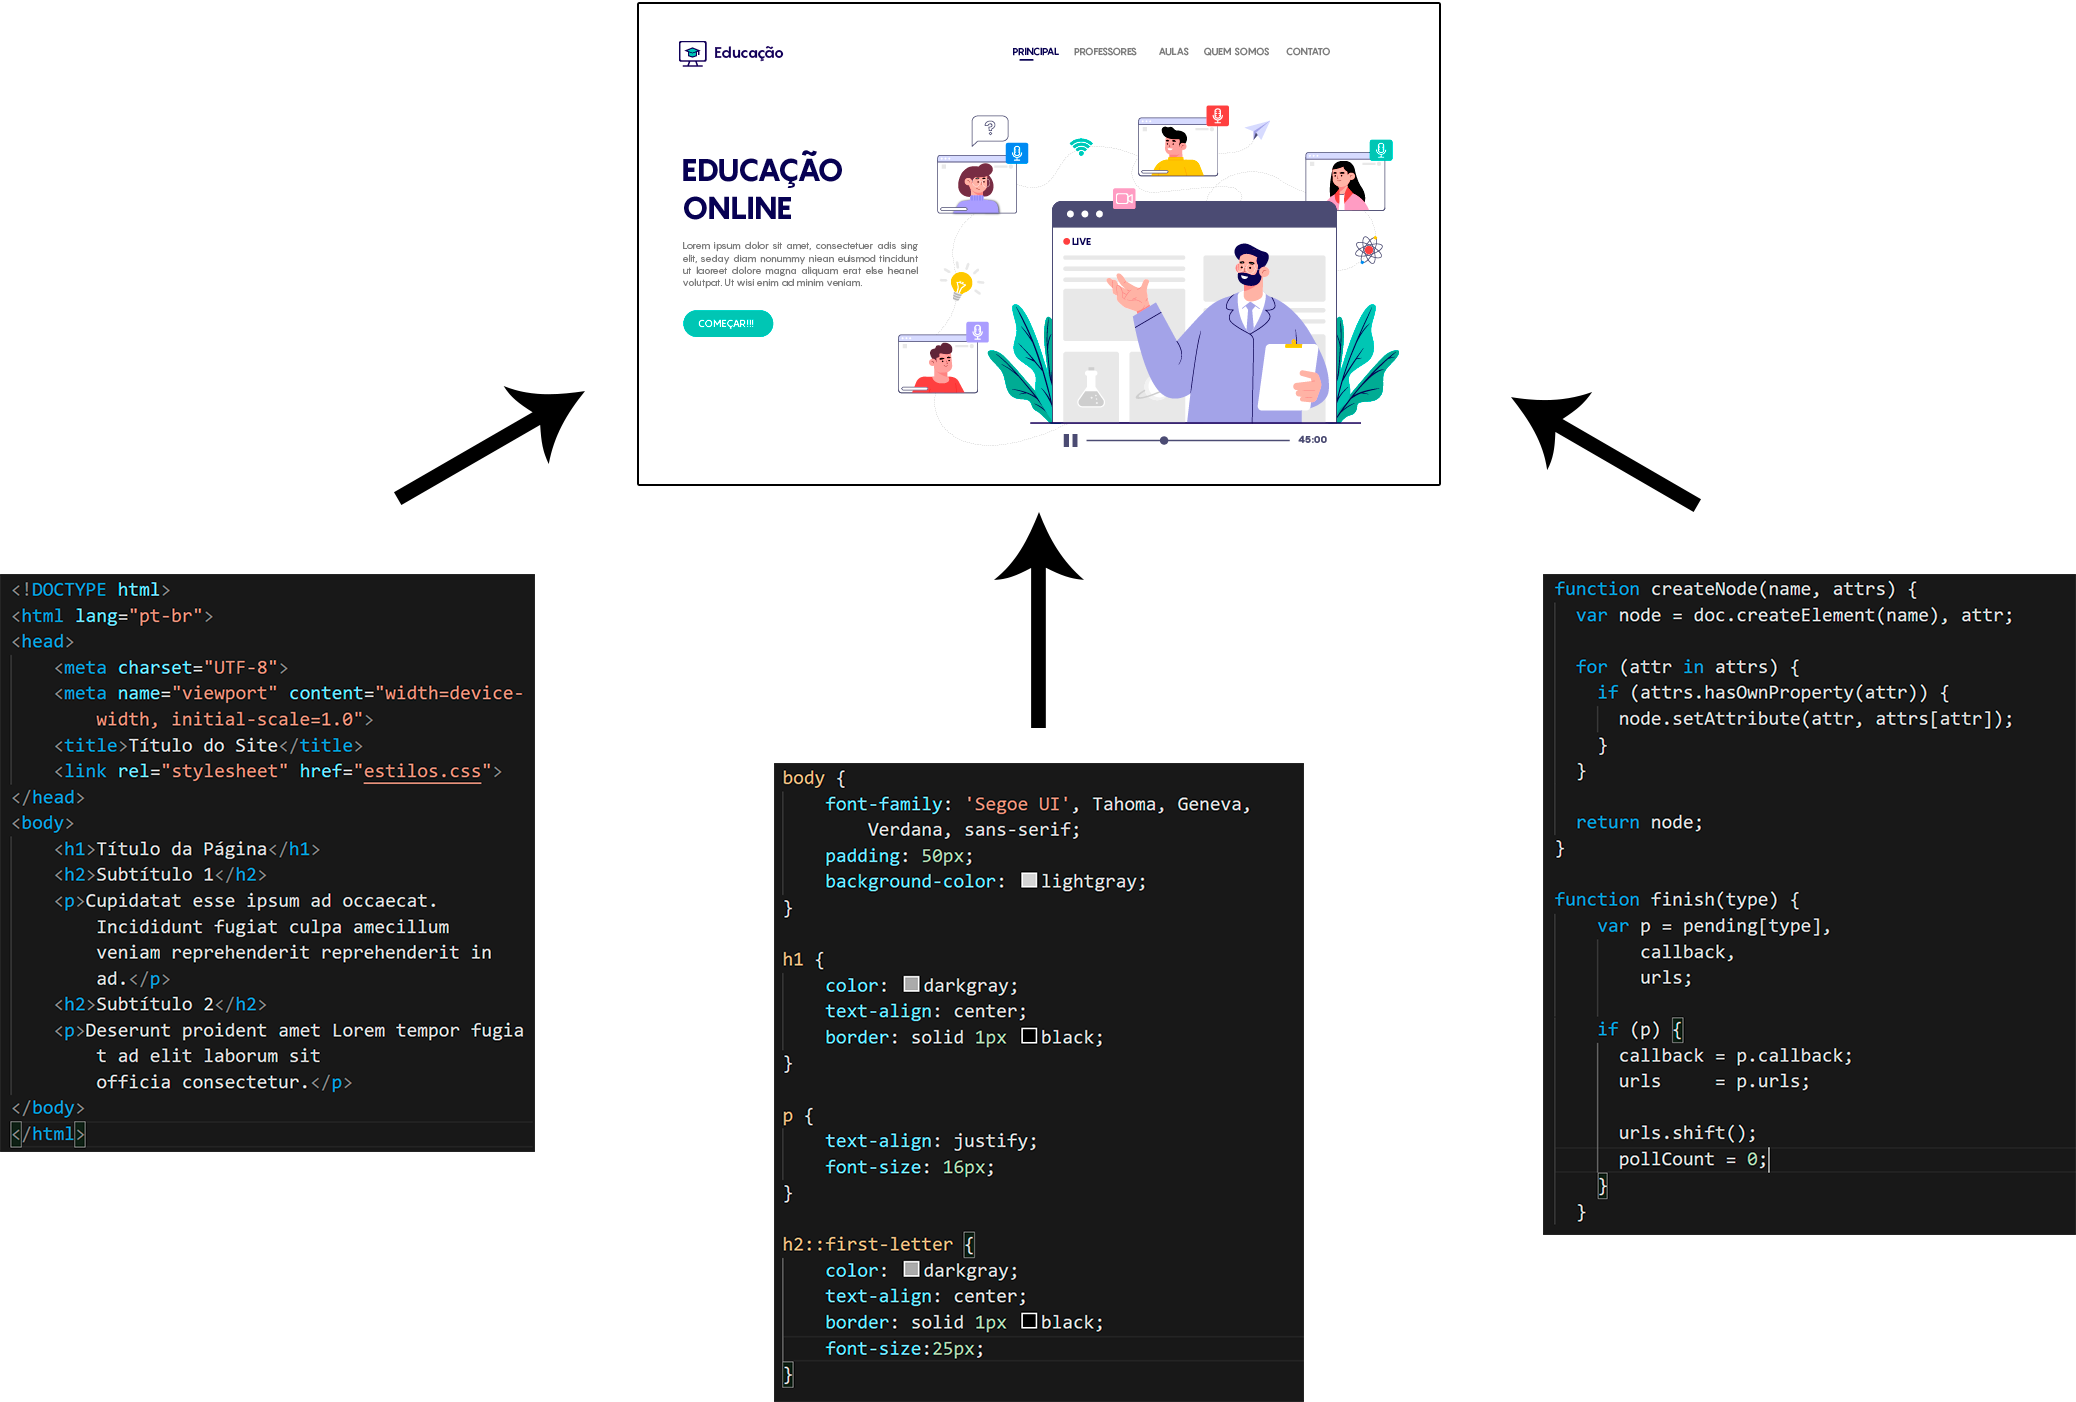
\includegraphics[width=1\textwidth]{Images/chapter01/site_codigos.png}
    \caption{Os códigos que compõem uma página de hipertexto.}
    \label{fig:sitescodigo}
\end{figure}

A primeira linguagem, \textbf{HTML}, é uma sigla para \textit{HyperText Markup Language}, traduzindo, Linguagem de Marcação de Hipertexto, ou seja, é uma linguagem de \textbf{marcação}. Em síntese, ela é a responsável por definir \textbf{quais} elementos serão exibidos em uma determinada página. \textbf{CSS} é outra sigla, que quer dizer \textit{Cascading Style Sheets}, ou folhas de estilo em cascata, portanto, é uma linguagem de \textbf{folhas de estilo}, ou uma linguagem de definição de estilos. Ela é responsável por definir \textbf{como} os elementos de conteúdo serão mostrados.

É através da linguagem CSS que apresentamos um mesmo conteúdo de forma alegre, de forma séria, de forma suave, chamativa etc. Resumindo, as definições de estilos CSS é que nos permitem mudar a forma como um conteúdo é exibido, ou seja, o visual do conteúdo.

Diferentemente de HTML e CSS, \textbf{Javascript} é uma linguagem de \textbf{programação}. Ela pode ter diferentes propósitos em uma página web e, pelo fato de ser uma linguagem de programação, requer conhecimentos de lógica de programação. Uma abordagem profunda da linguagem Javascript está fora do escopo deste material. Veremos apenas qual é o papel da linguagem Javascript em uma página web.

Primeiramente, é importante ressaltar que, para construir sites, não somos obrigados a usar Javascript. Na verdade, basicamente, somente sites que possuem interação com o usuário e/ou efeitos visuais avançados é que requerem o uso de Javascript . No final deste capítulo, eu voltarei a falar um pouco mais sobre Javascript, só para dizer como ele pode contribuir para o funcionamento de um site. Temos que ver algumas coisas antes para que você entenda melhor o papel do código Javascript.

Bem, essa combinação de HTML, CSS e Javascript forma o código-fonte de uma página web. Você consegue ver o código-fonte de qualquer página web clicando com o botão direito do mouse sobre a página em um navegador qualquer e selecionando a opção “Exibir código-fonte da página”, ou “Ver código-fonte da página”, ou alguma coisa parecida com isso (depende do navegador). 

A princípio, o código-fonte que será exibido pode parecer algo meio assustador, mas em pouco tempo você já será capaz de compreender boa parte dele. O código-fonte de uma página web geralmente fica distribuído em mais de um arquivo. Na verdade, é uma boa prática separar em arquivos distintos os códigos HTML, CSS e Javascript. Pode acontecer, inclusive, de cada tipo de arquivo ser mantido por um programador diferente.

Normalmente, uma página contém apenas 1 arquivo HTML, mas pode estar associada a vários arquivos CSS e a vários arquivos Javascript. Os arquivos HTML podem ter a extensão ``htm'' ou ``html'', enquanto os arquivos CSS possuem a extensão ``css'', e os arquivos Javascript possuem a extensão ``.js''.

Quanto ao código CSS, é comum ter um arquivo para estilizar botões, outro para estilizar o leiaute da página, outro para estilizar os textos, entre outros mais. Separar esses códigos CSS em arquivos diferentes pode ajudar a melhorar a organização do código-fonte de um site como um todo. Portanto você poderia criar um arquivo CSS para estilizar botões, outro para o leiaute, outro para a tipografia e assim por diante.

Outra observação importante é que as páginas de um mesmo site normalmente possuem um mesmo estilo. Geralmente usam as mesmas cores, a mesma tipografia, o mesmo leiaute, o mesmo estilo de cabeçalho e rodapé, entre outras coisas. Portanto, é comum que os mesmos arquivos CSS sejam compartilhados entre diferentes páginas web.

Assim, se você quiser mudar a tipografia usada em todas as páginas do site, basta ir ao arquivo CSS que contém essa formatação e mudar as propriedades de fonte desejadas. Assim, o site inteiro passará a ser mostrado com as novas definições de fonte. Pense em como isso facilita a manutenção de um site!

Quanto ao código Javascript, também é comum que as páginas compartilhem os mesmos códigos. É possível ter um código para mostrar uma janela com mensagem, para animar um elemento da página, para atualizar apenas uma parte da página, entre outros. Se determinado código Javascript é específico de uma página, recomenda-se separá-lo em um arquivo que será vinculado exclusivamente à página a que pertence. Isso evita que outras páginas carreguem códigos Javascript que não sejam necessários para ela. Assim como ocorre com CSS, é comum que um mesmo arquivo Javascript esteja vinculado a diferentes páginas, pois elas podem ter funcionalidades comportamentais em comum.

\subsection{Páginas Estáticas e Dinâmicas}

Os arquivos que compõem o código-fonte de uma página podem ter origem de duas fontes diferentes: podem ser arquivos prontos, que simplesmente serão baixados do servidor web que hospeda o site; ou podem ser gerados por um programa especial chamado de aplicação web, que roda no servidor web e que gera o código-fonte da página sempre que ela é solicitada por um usuário.

Quando as páginas de um site são totalmente compostas por arquivos prontos, dizemos que o site é estático. Quando as páginas (ao menos algumas delas) são geradas por uma aplicação web, dizemos que o site é dinâmico. É muito comum ter sites que possuem páginas estáticas e páginas dinâmicas. A figura \ref{fig:sitesestdyn} mostra como os sites estáticos e dinâmicos são servidos ao navegador do usuário.

\begin{figure}[htbp!]
    \centering
    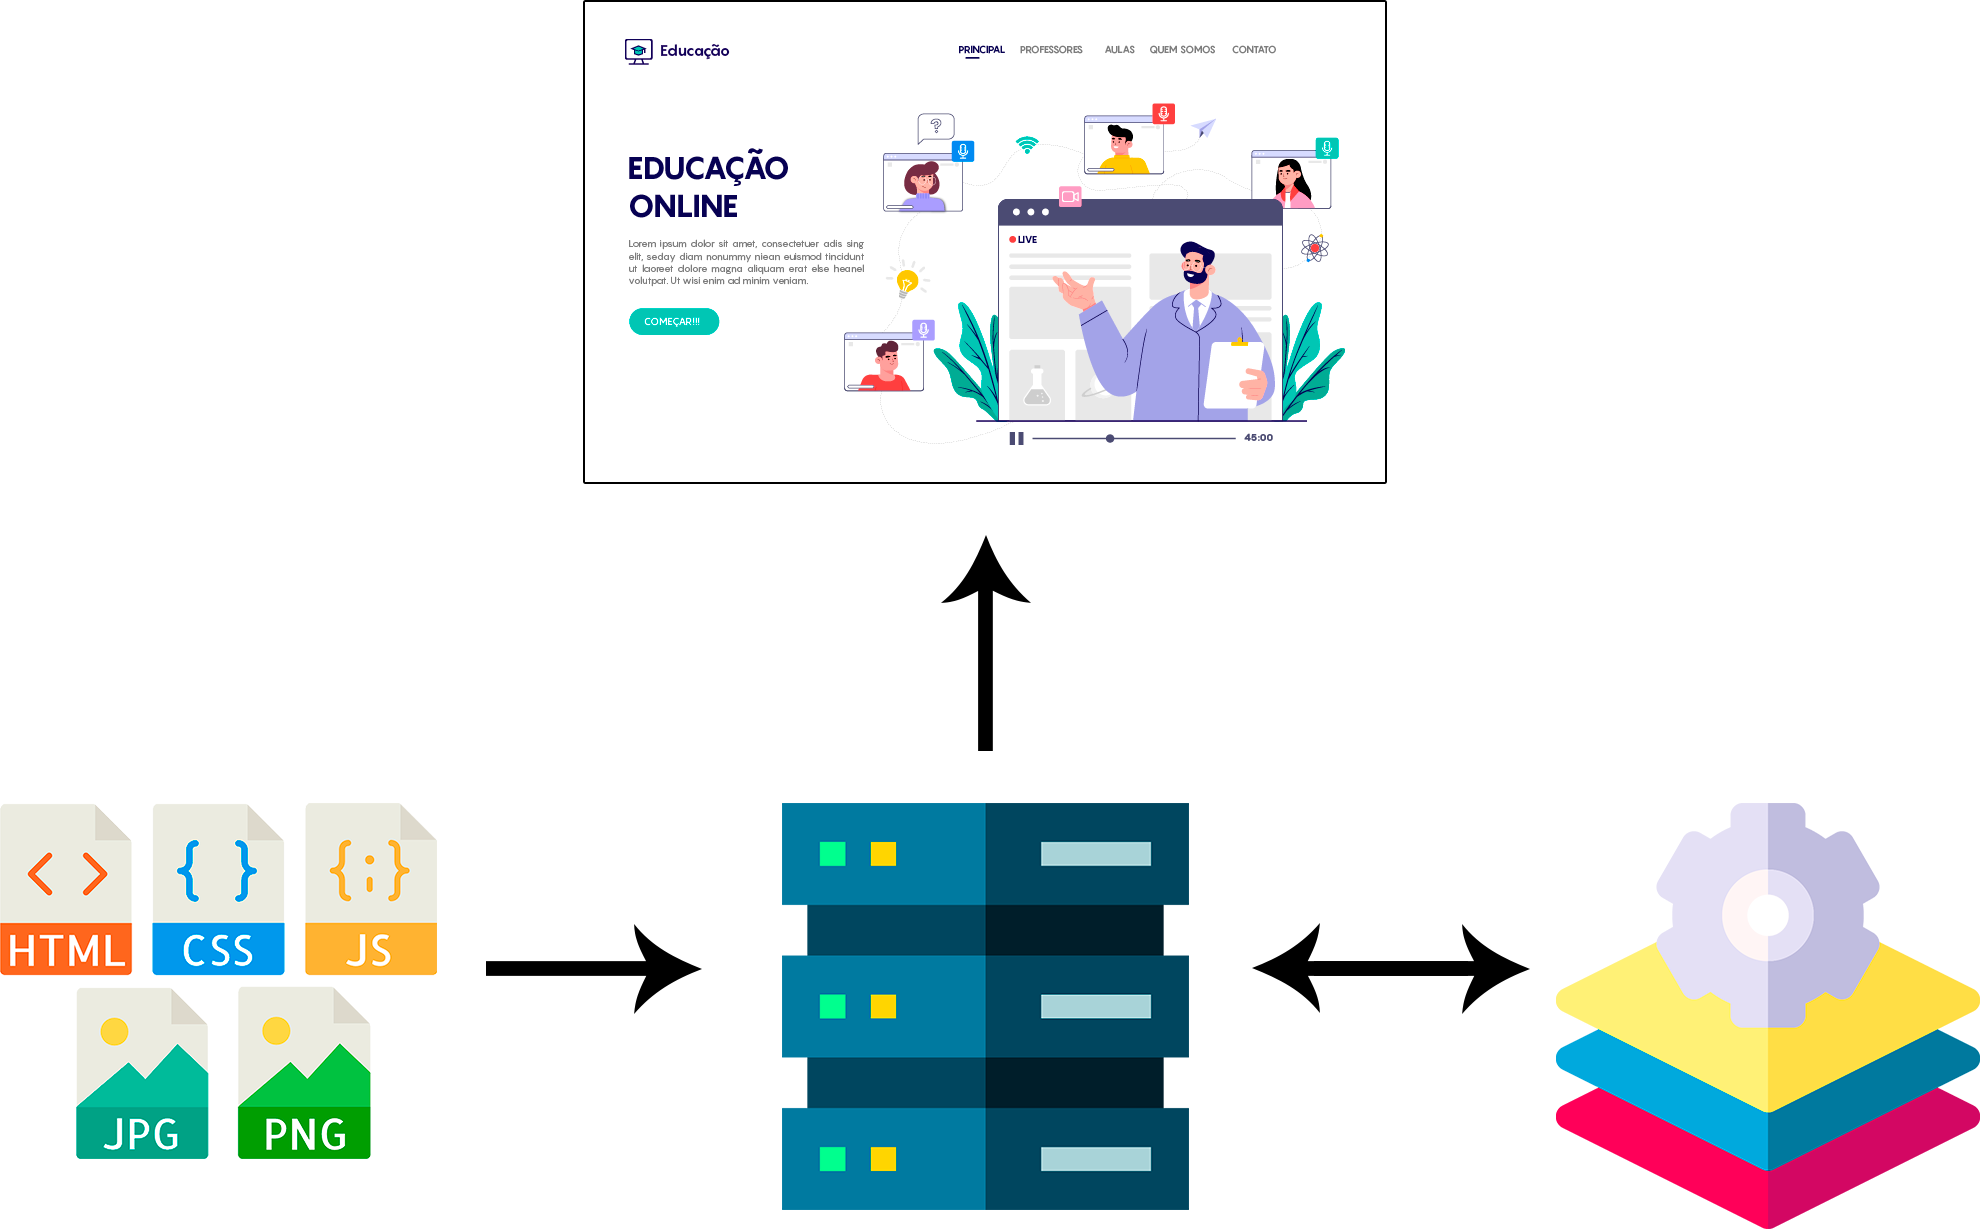
\includegraphics[width=1\textwidth]{Images/chapter01/site_est_dyn.png}
    \caption{Sites estáticos e dinâmicos.}
    \label{fig:sitesestdyn}
\end{figure}

Normalmente, o código que é gerado dinamicamente por uma aplicação web é aquele relacionado ao conteúdo da página, ou seja, o código HTML. Os códigos CSS e Javascript raramente são gerados dinamicamente. Normalmente eles são criados de forma estática por um programador e permanecem intocados ao longo de toda a vida da aplicação web. Quando é necessário atualizar a aparência do site ou incluir novas funções Javascript para executar alguma tarefa adicional, os arquivos podem ser modificados por alguém, mas depois da modificação eles continuam estáticos no servidor, ou seja, eles \textbf{não serão gerados} pela aplicação web.

Um site estático tem a característica de não demandar atualizações com muita frequência. Um site que tenha o propósito de contar a história do Brasil, por exemplo, vai ter um conteúdo que dificilmente será alterado. Se houver necessidade de alteração, a frequência será tão baixa que basta fazer a alteração diretamente nos arquivos HTML. Não vale a pena criar uma aplicação web acessando um banco de dados para gerar conteúdo se tal conteúdo muda somente uma vez por ano, por exemplo. Neste caso, vale a pena abrir o arquivo HTML em um editor e fazer a modificação diretamente no arquivo correspondente ao conteúdo da página. 

\subsection{O Conceito de Requisição de Página}

Quando um endereço de um site é digitado na barra de endereços do navegador, a primeira coisa a ser baixada pelo navegador é o código HTML. Como já mencionado, esse código pode vir de um arquivo estático ou pode ser gerado por uma aplicação web que esteja rodando no servidor. Esse código HTML normalmente contém referências para os demais arquivos necessários para a página ser renderizada. Aí entram os arquivos com códigos CSS e Javascript, os arquivos de imagens e arquivos de outras mídias que façam parte da página. De posse do endereço desses arquivos associados, o navegador faz o download de cada um deles e renderiza a página.

A figura \ref{fig:reqpagina} apresenta um diagrama que mostra desde o momento em que o usuário digita o endereço de um site no navegador até o momento em que o navegador exibe a página para o usuário. Ressalto que esse diagrama é uma abstração do processo real. Isso quer dizer que algumas detalhes que acontecem nos bastidores foram suprimidos ou simplificados visando facilitar o entendimento do processo.

\begin{figure}[htbp!]
    \centering
    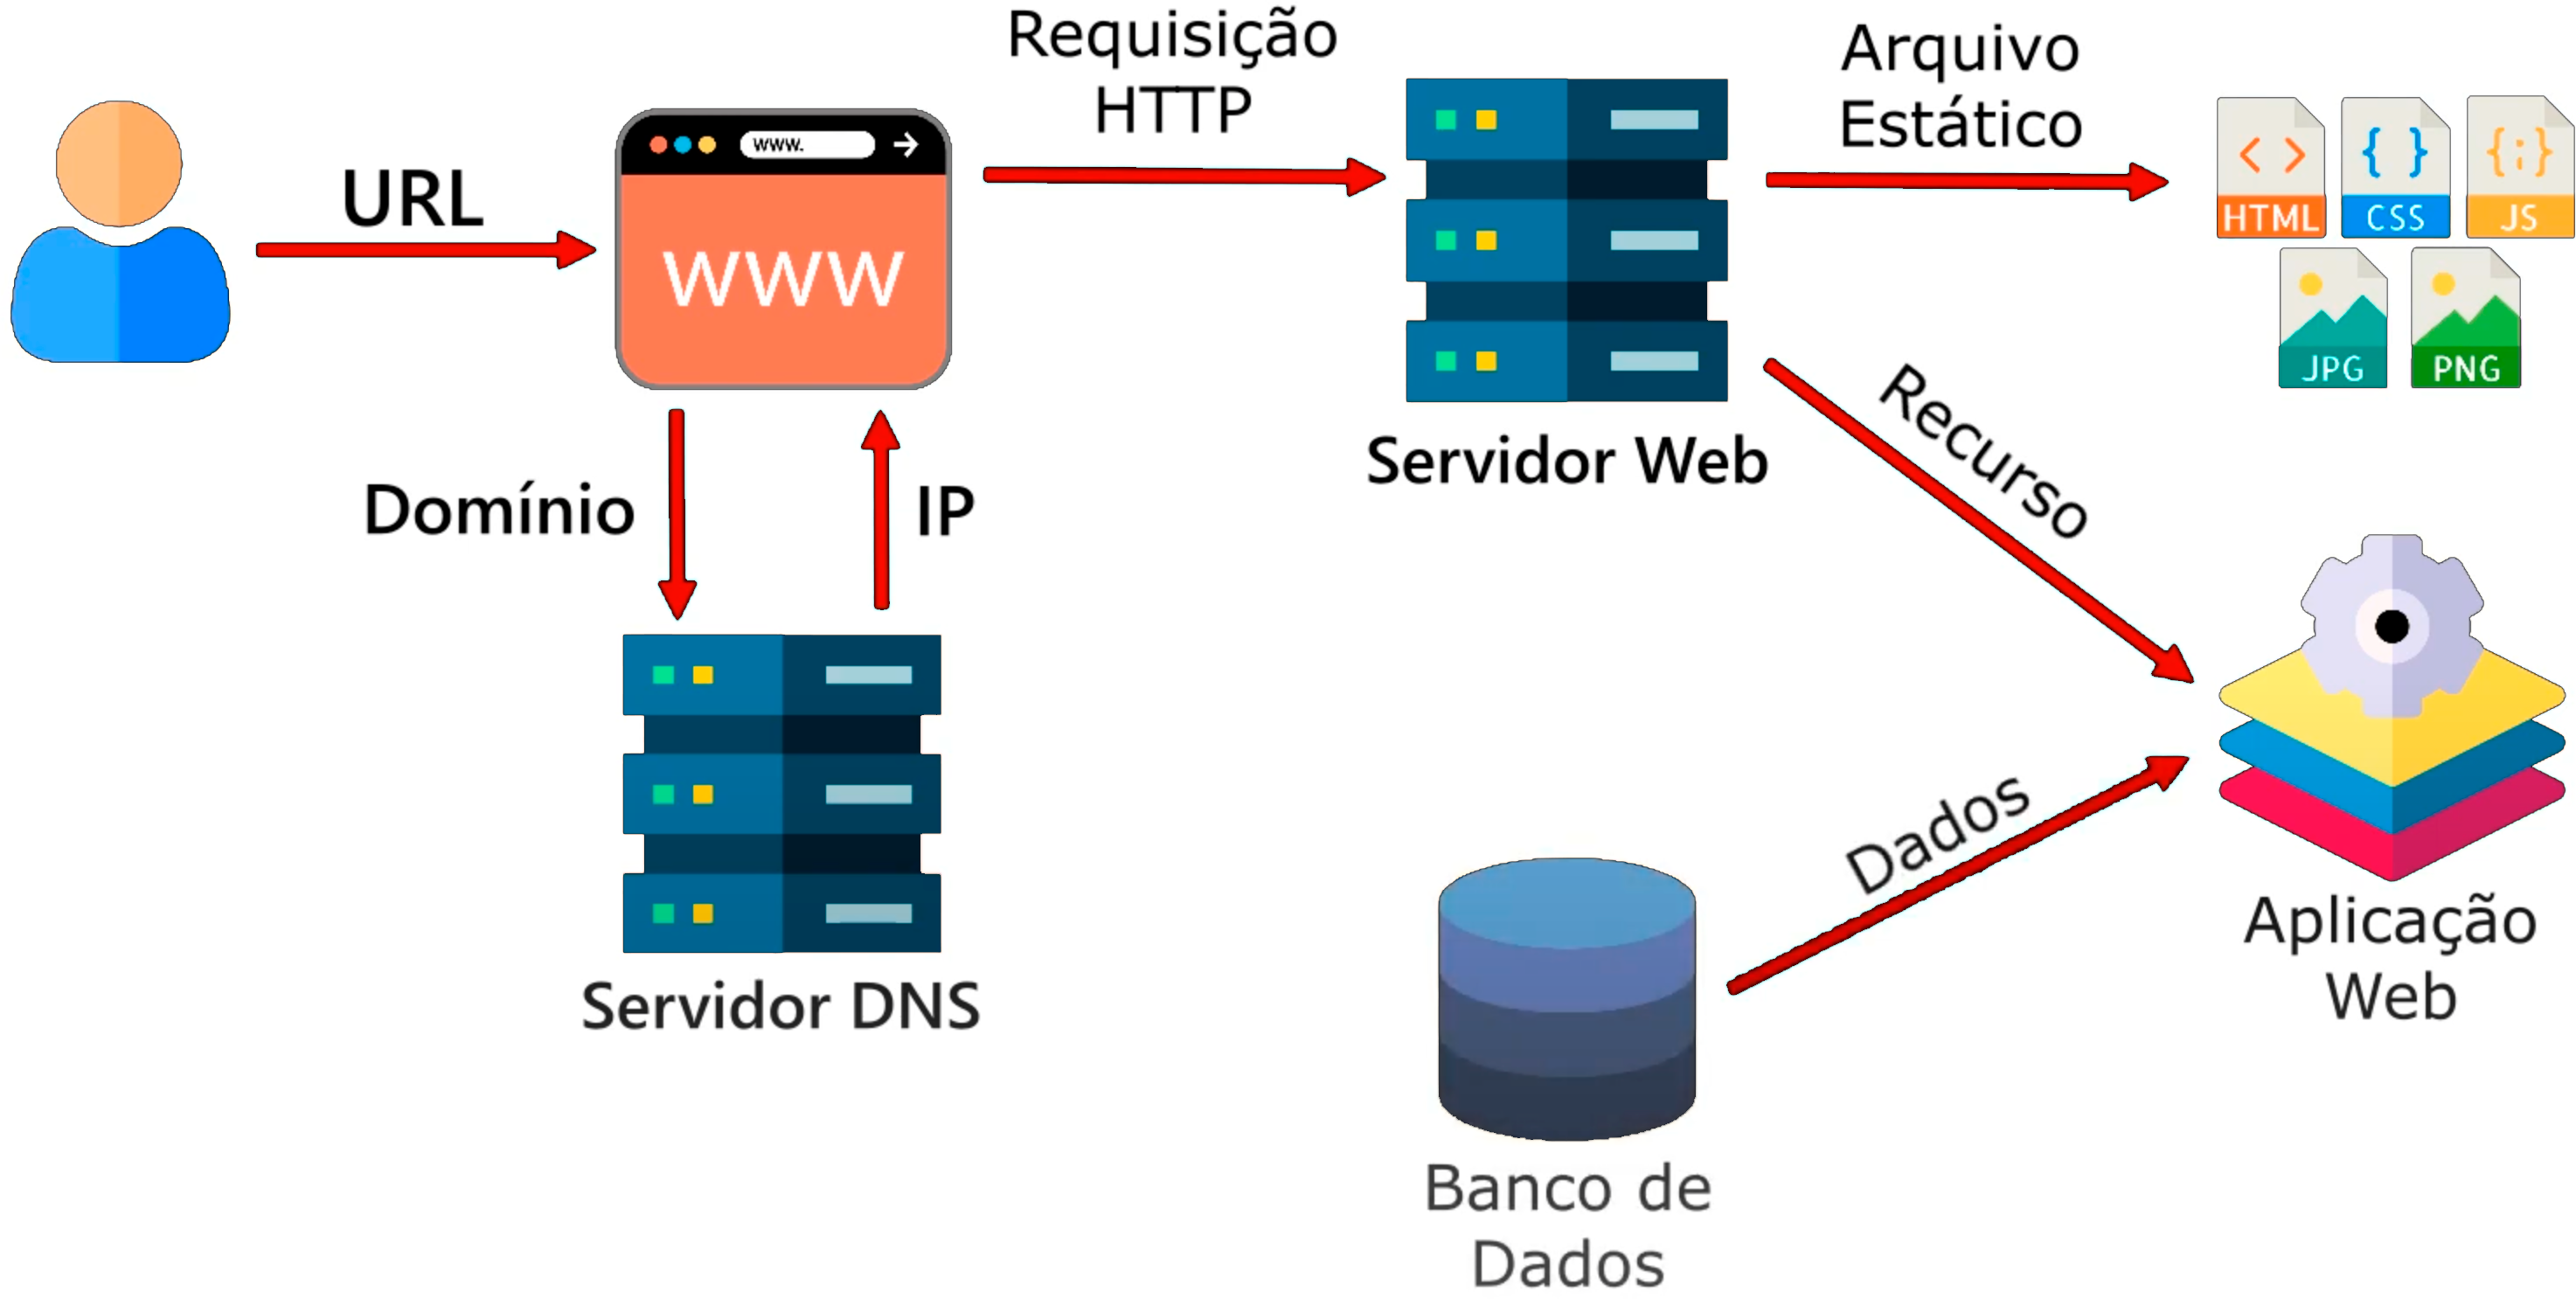
\includegraphics[width=1\textwidth]{Images/chapter01/digrama_requisicao.png}
    \caption{Diagrama de uma requisição de página pelo navegador.}
    \label{fig:reqpagina}
\end{figure}

Na figura \ref{fig:reqpagina}, tudo começa com o usuário informando uma URL na barra de endereços do navegador. Acontece que, para acessar um servidor web, é necessário saber seu número IP. A sigla IP vem de \textit{Internet Protocol}, ou ``protocolo de internet''. O número IP de um servidor é mundialmente único, ou seja, ele é um endereço exclusivo do servidor em toda a internet.

Os nomes de domínio, como google.com.br, maroquio.com.br e youtube.com.br, são simplesmente apelidos para endereços IP de um servidor. O fato de usarmos nomes de domínio em vez de endereços IP numéricos é pelo fato dos nomes serem humanamente mais fáceis de se memorizar e mais fáceis de serem associados a entidades do mundo real. Em síntese, além de ser mais fácil memorizar um nome do que um número que pode ter até 12 dígitos, o nome do domínio pode ser composto pelo próprio nome da entidade que ele representa, facilitando ainda mais a memorização. O domínio microsoft.com é um exemplo disso.

Mas como o navegador faz para descobrir o endereço IP de um servidor web a partir de um nome de domínio? Na verdade, o navegador consulta primeiro um servidor DNS. DNS significa \textit{Domain Name System}, ou ``Sistema de Nomes de Domínios''. Esse servidor contém uma tabela que mapeia nomes de domínios para endereços IP. Portanto, quando ele recebe um pedido de consulta de um domínio, ele percorre essa tabela e retorna o IP do domínio consultado.

Existem vários servidores DNS espalhados pelo mundo, e essa tabela é atualizada com certa frequência para refletir a inclusão de novos domínios que tenham sido registrados, bem como a remoção de domínios que não estão mais ativos e a alteração de domínios que ocorre quando um site é mudado de um servidor web para outro.

Uma vez que o endereço IP do servidor web tenha sido obtido, uma requisição HTTP é feita ao servidor web correspondente ao IP em questão. Não se assuste com o termo ``requisição HTTP''. Isso nada mais é do que o seu navegador fazendo um pedido de algum recurso para o servidor web usando uma linguagem que os dois conhecem bem, que é o protocolo \textbf{HTTP}. 

A sigla HTTP, que você já deve ter visto no início do endereço de vários sites, quer dizer \textit{Hyper Text Transfer Protocol}, ou, ``Protocolo de Transferência de Hipertexto''. Lembra que eu falei que as páginas de um site são hipertextos? Pois é! Por isso o nome do protocolo diz respeito à transferência de hipertexto.

Existe uma forma correta de o navegador solicitar uma página de hipertexto a um servidor web. Essa forma é o que chamamos de ``protocolo'', que neste caso é o HTTP. Uma requisição HTTP é composta por vários dados, entre eles, o idioma preferencial do usuário, o nome de domínio onde está o recurso solicitado e o nome do recurso que está sendo solicitado. O recurso solicitado por ser um arquivo HTML, CSS, Javascript, ou pode ser um arquivo de imagem qualquer, ou, pode ser um nome de recurso que será gerado por uma aplicação web. O código \ref{code_req} mostra um exemplo de cabeçalho HTTP para uma requisição ao servidor da Microsoft.

\begin{htmlcode}{Exemplo de cabeçalho de uma requisição HTTP}{code_req}
GET /produtos HTTP/1.1
Host: www.microsoft.com
User-Agent: Mozilla/5.0 (Windows NT 10.0; Win64; x64) Chrome/89.0.4389.82 Safari/537.36
Accept: text/html,application/xhtml+xml,application/xml;q=0.9,image/webp,*/*;q=0.8
Accept-Language: en-US,en;q=0.5
Accept-Encoding: gzip, deflate, br
Connection: keep-alive
\end{htmlcode}


Cada arquivo necessário para a renderização da página gera uma requisição HTTP. Veja que isso tudo acontece em poucos segundos. Lembre-se também de que, quanto menor é o tempo de carregamento de uma página, menos chance ela tem de ser abandonada pelo usuário. Um dos maiores desafios ao se construir um site é o de reduzir o tempo de carregamento das páginas. Ao longo deste material, veremos algumas técnicas que vão ajudar nessa questão.

Continuando no diagrama da figura \ref{fig:reqpagina}, vamos imaginar que o recurso solicitado é uma página dinâmica. Nesse caso, para gerar a página, alguns dados a mais normalmente são necessários, e esses dados costumam ficar armazenados em um banco de dados. Vamos analisar um exemplo real rapidamente. 

A figura \ref{fig:pagsyout} mostra as páginas com detalhes de 3 vídeos do meu canal no YouTube, cada uma com seu respectivo endereço. Veja que os endereços são bem parecidos. Todos começam com HTTPS, que nada mais é do que uma versão segura do protocolo HTTP. Em seguida vem o nome do domínio, nesse caso, \textit{www.youtube.com}. Depois vem o nome do recurso que estamos acessando, que é a página \textit{watch}; e, por fim, temos uma interrogação (?) seguida de um ``V=XXXXXXX'', onde o \textit{X} pode ser qualquer caractere alfanumérico. 

\begin{figure}[htbp!]
    \centering
    
\includegraphics[width=1\textwidth]{Images/chapter01/pags_youtube1.png}
    \caption{Páginas de vídeos específicos do YouTube.}
    \label{fig:pagsyout}
\end{figure}

Isso que vem depois da interrogação na URL do vídeo é um parâmetro. Esse parâmetro é o identificador do vídeo que está sendo exibido. É como se fosse o ``CPF'' do vídeo. Daqui a pouco vamos estudar mais sobre esse identificador. Veja que o estilo da página é o mesmo para os três vídeos. Isso caracteriza bem as páginas geradas dinamicamente. Elas têm um estilo praticamente idêntico, incluindo fonte de letra, cores, leiaute, botões etc., e alguns dados mudam de uma para outra.

Tente identificar, na figura \ref{fig:pagsyout}, quais dados mudam de uma página para outra. Vamos lá. Temos a imagem de capa do vídeo, o título, a quantidade de visualizações, a data de publicação, a quantidade de likes e dislikes, e a descrição. Esses dados são obtidos de um banco de dados no servidor do YouTube. Se você nunca estudou banco de dados, não se preocupe, porque é algo desnecessário para esta fase do aprendizado. A figura \ref{fig:pagsyoutmarcado} mostra os dados dinâmicos contornados por retângulos alaranjados.

\begin{figure}[htbp!]
    \centering
    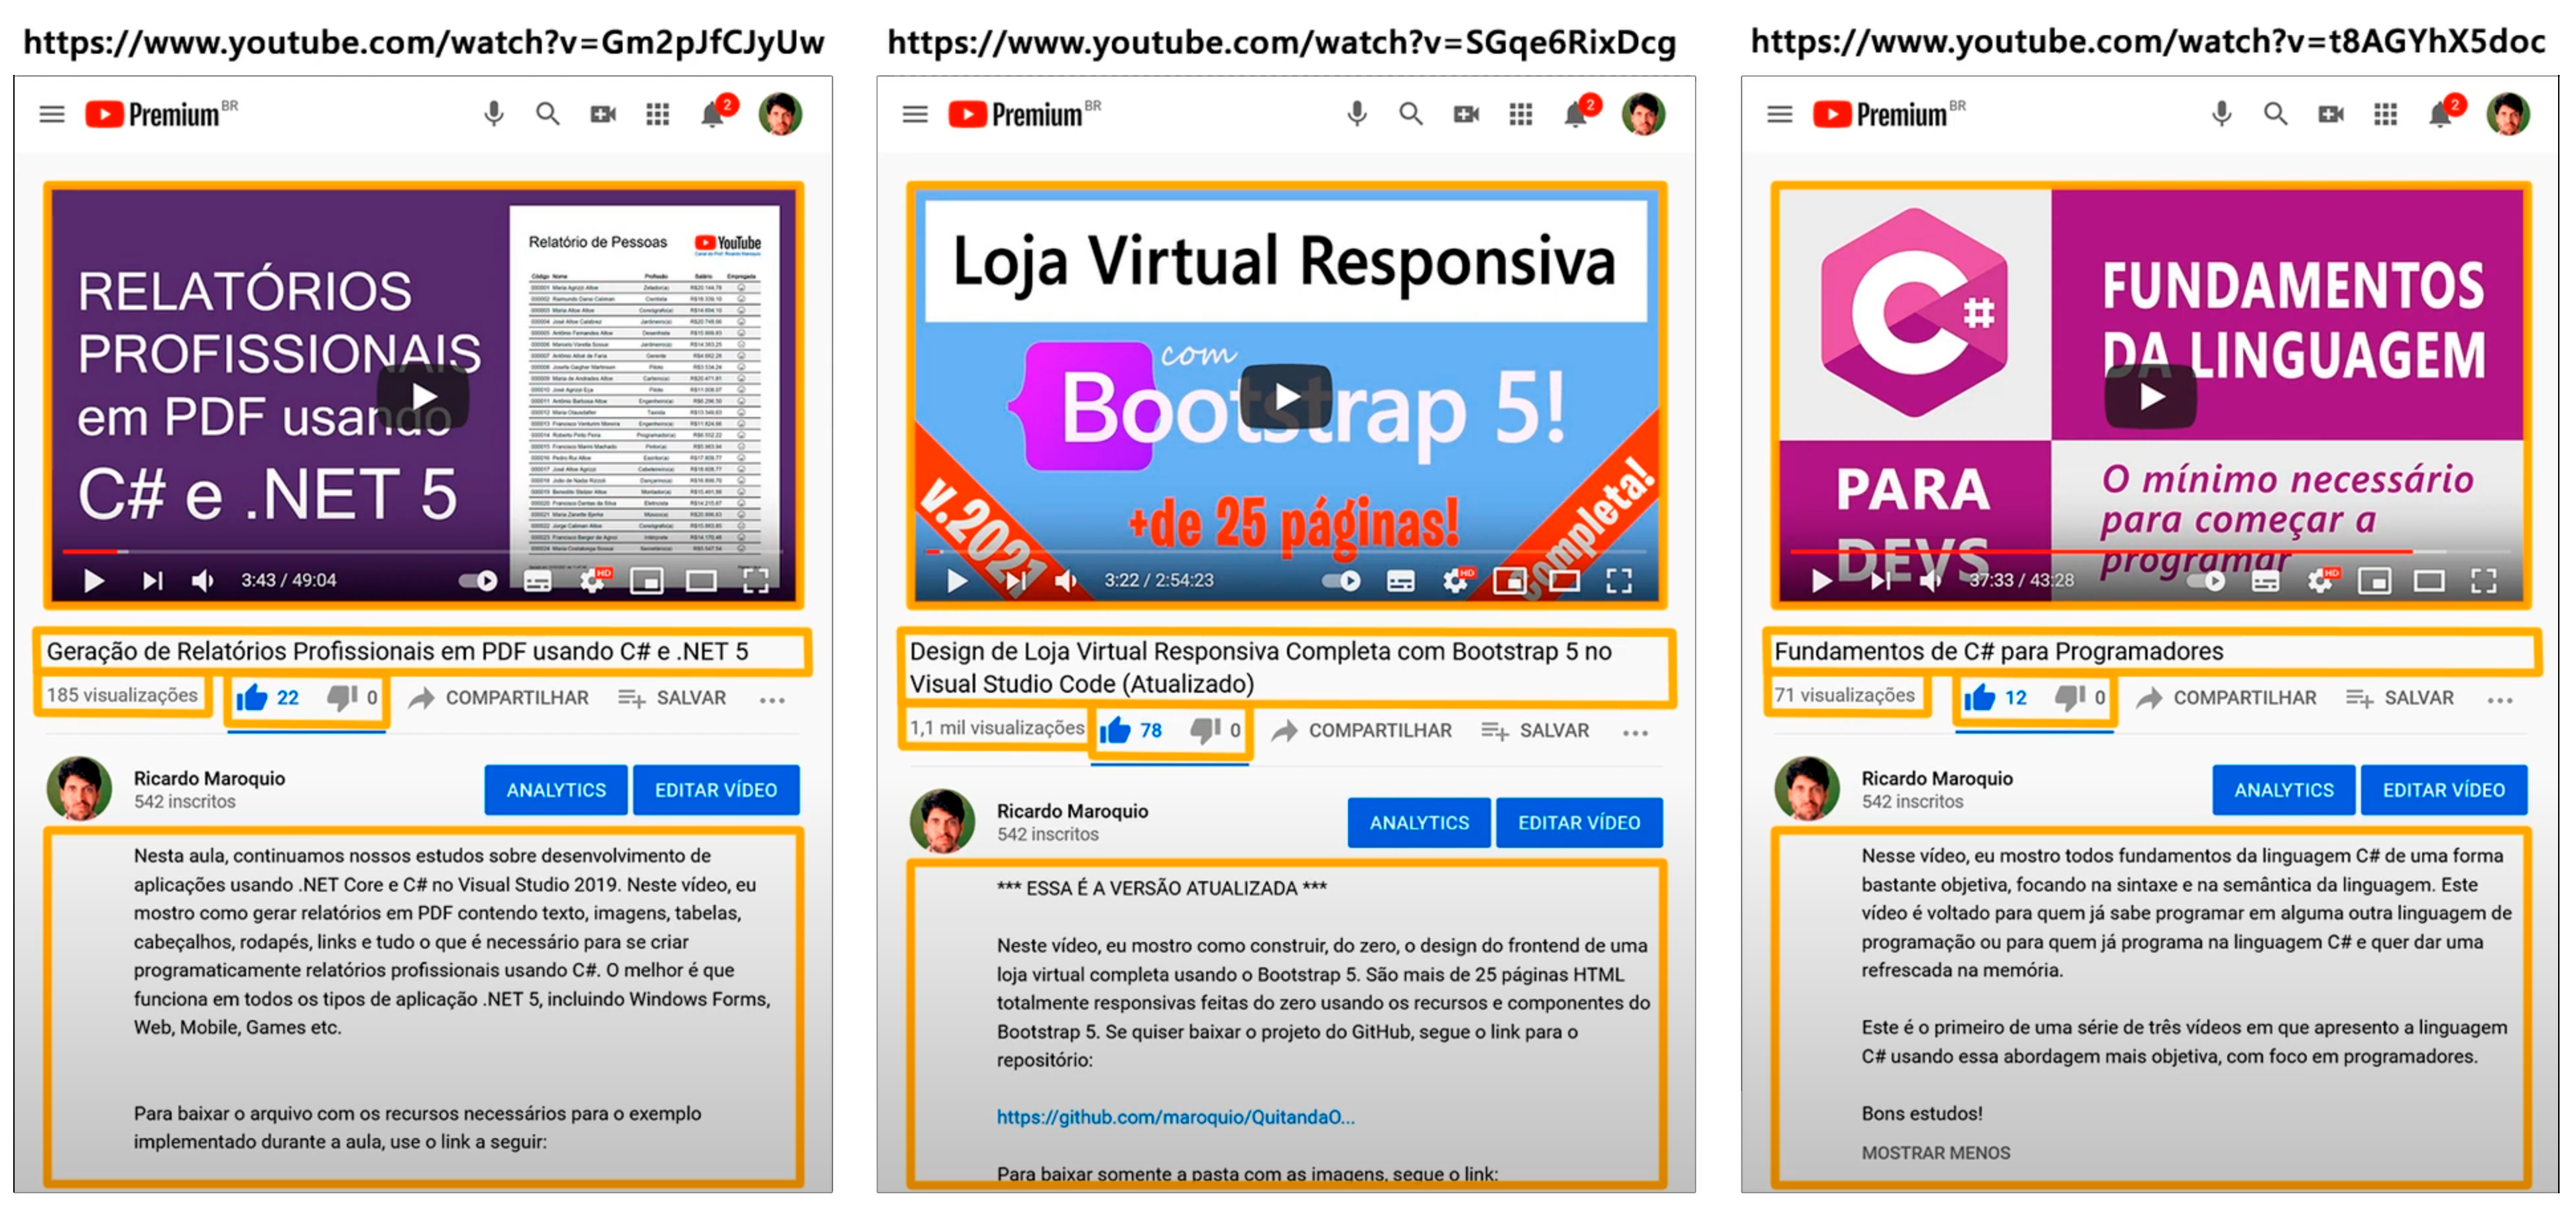
\includegraphics[width=1\textwidth]{Images/chapter01/pags_youtube2.png}
    \caption{Páginas de vídeos específicos do YouTube com dados dinâmicos destacados.}
    \label{fig:pagsyoutmarcado}
\end{figure}

Tudo que vem depois de uma interrogação em uma URL é considerado parâmetro. Pode acontecer de uma mesma URL ter vários parâmetros separados pelo símbolo \textbf{\&}. O valor desse parâmetro ``V'' funciona como um identificador. Com ele é possível encontrar um determinado vídeo no banco dados de vídeos do YouTube. Se você já estudou banco de dados, já deve ter feito a associação desse parâmetro ``V'' com a chave primária de uma tabela que guarda os dados dos vídeos.

A aplicação web do YouTube foi programada para usar esse parâmetro e consultar um banco de dados para buscar os dados específicos do vídeo em questão. Em seguida, a aplicação web combinou esses dados com um modelo genérico de página HTML criado por algum designer do YouTube, gerando o conteúdo e enviando de volta ao navegador do usuário através de uma resposta HTTP. 

Esse modelo de página HTML já contém as referências para arquivos CSS, Javascript, imagens e o que mais for necessário para renderizar a página do vídeo por completo. Portanto, conforme já estudamos, logo que recebe esse conteúdo HTML, o navegador já faz novas requisições ao servidor do YouTube para buscar os outros arquivos necessários para a renderização da página. Depois de baixar todos os arquivos, a renderização da página é concluída.

\subsection{Um Pouco Mais Sobre Javascript}

Agora vamos voltar a falar do código Javascript que vimos rapidamente. Basicamente, ele desempenha dois papéis em uma página de hipertexto. O primeiro deles é a modificação de conteúdo mediante a ocorrência de algum evento. Por exemplo, se o usuário clicar em um botão, eu quero que determinado menu seja expandido ou que uma imagem sofra um zoom. Isso quer dizer que, com Javascript, você consegue manipular os elementos HTML que estão renderizados em uma página, incluindo seus estilos CSS. Isso pode deixar a página um pouco mais interativa.

O segundo papel desempenhado pelo Javascript é o de carregar conteúdo do servidor web em segundo plano, permitindo atualizar partes da página sem a necessidade de requisitar toda a página novamente. Como exemplo, imagine um site que mostre o placar de jogos de futebol em tempo real, como na figura \ref{fig:site_placar}. Para que a experiência do usuário seja a melhor possível, é interessante atualizar o placar no máximo a cada 1 segundo, senão o usuário escuta o grito de gol do vizinho e só 30 segundos depois o placar muda para ele, gerando uma péssima experiência.

\begin{figure}[htbp!]
    \centering
    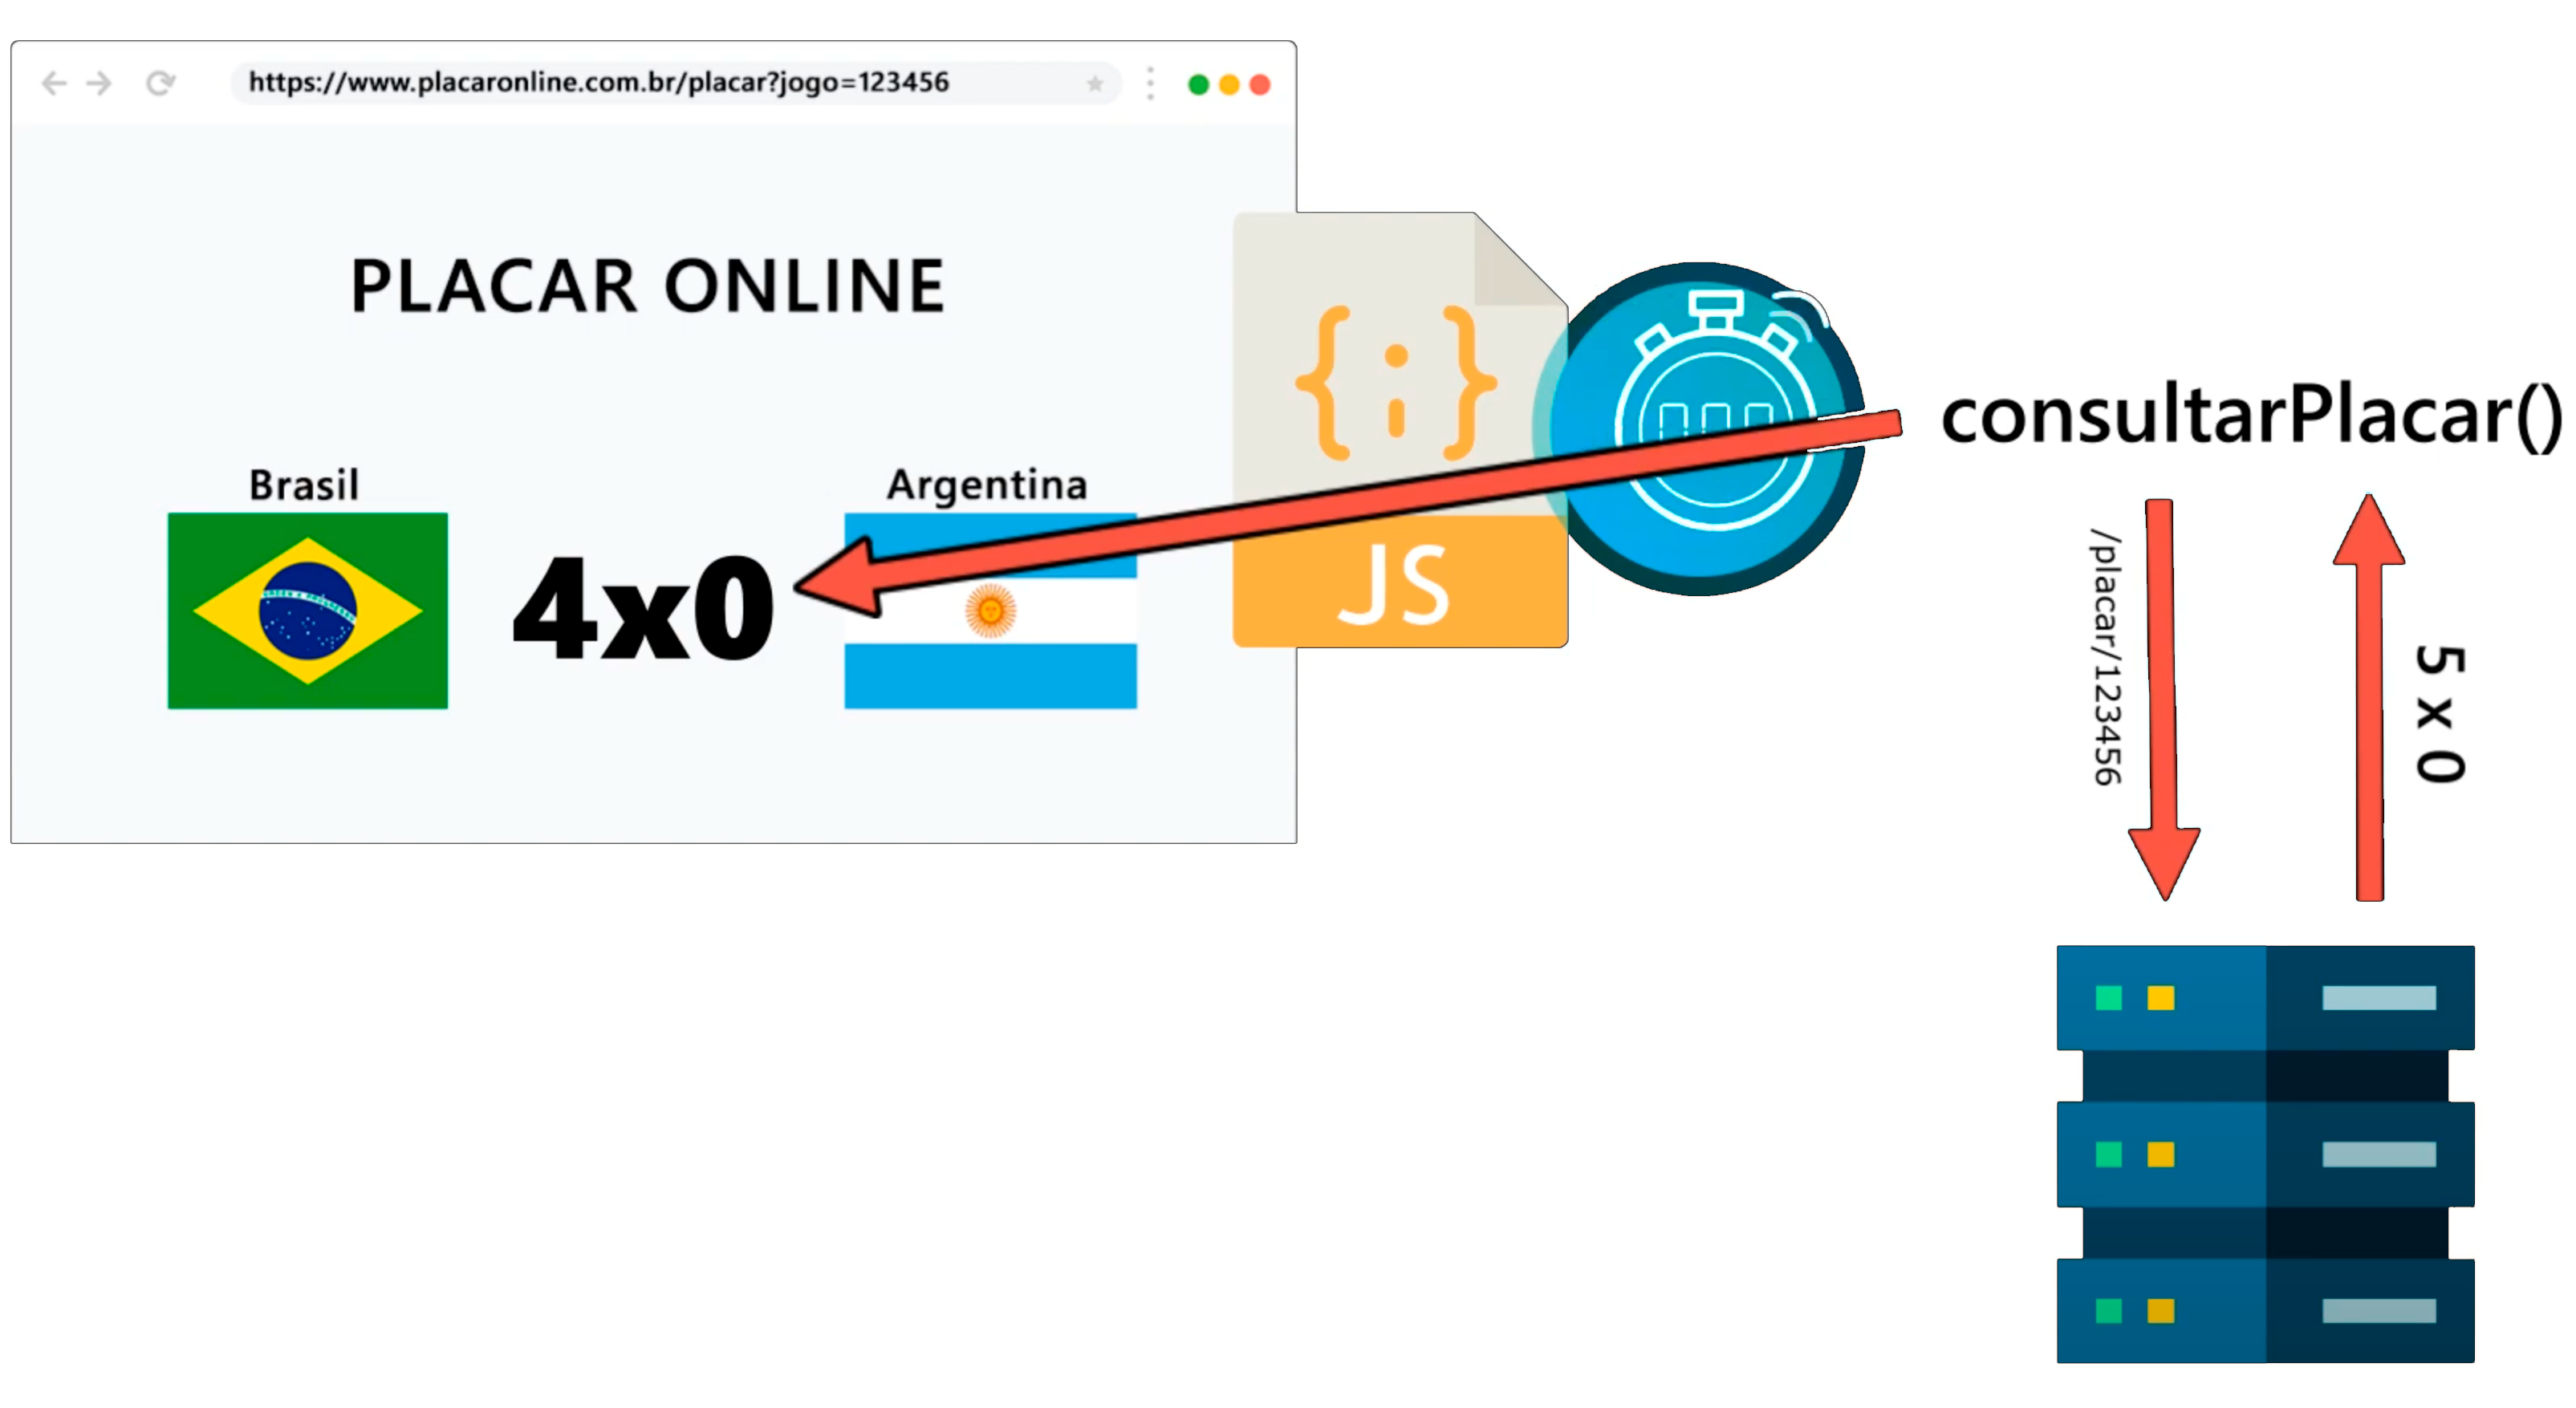
\includegraphics[width=1\textwidth]{Images/chapter01/site_placar.png}
    \caption{Atualização parcial de página usando Javascript em segundo plano.}
    \label{fig:site_placar}
\end{figure}

Acontece que recarregar toda a página novamente a cada segundo é algo computacionalmente custoso, e milhares de usuários fazendo isso ao mesmo tempo sobrecarregaria o servidor. Neste caso, usando Javascript, é possível criar um temporizador que dispare uma função a cada 1 segundo, sendo que essa função faz uma consulta ao servidor web usando o endereço de um recurso que retorna somente o placar do jogo em questão. Em seguida, a função vai no elemento HTML que mostra o placar na página e atualiza seu conteúdo com o novo valor do placar recebido do servidor. Isso tudo é realizado em segundo plano pelo navegador e evita o recarregamento total da página.

Apesar de Javascript ser um recurso útil, principalmente para a criação de sites dinâmicos, o foco deste material é a criação de sites estáticos. Na verdade, independentemente do site ser estático ou dinâmico, o código que chega no navegador para ser renderizado tem exatamente as mesmas características, ou seja, tipicamente temos o código HTML para definir o conteúdo e o código CSS para definir a aparência do site. Eventualmente, podemos ter código Javascript para desempenhar algum dos papéis que mencionei. Isso quer dizer que, para criar sites dinâmicos, o primeiro passo é aprender a criar sites estáticos, que é o nosso propósito aqui.

\section{Exercícios Propostos}

Essa série de exercícios envolve os conceitos abordados neste capítulo e também \textbf{pode demandar alguma pesquisa}. Reserve um tempo e um local adequados para fazer os exercícios sem distrações. Assim você absorverá muito mais o conteúdo estudado.

\begin{exercise}
Quais são os 3 tipos de códigos básicos de uma página de hipertexto? Explique para que serve cada um dos tipos.
%R: Os três tipos de códigos básicos de uma página de hipertexto são HTML (HyperText Markup Language), CSS (Cascading Style Sheets) e JavaScript. O HTML define a estrutura e o conteúdo da página, o CSS define a aparência visual da página e o JavaScript permite a criação de interações e funcionalidades dinâmicas na página.
\end{exercise}

\begin{exercise}
Quantos arquivos CSS e Javascript podem estar vinculados a uma mesma página de hipertexto? Justifique sua resposta.
%R: Não há um número máximo ou mínimo de arquivos CSS e JavaScript que podem estar vinculados a uma página de hipertexto. Depende da complexidade da página e da quantidade de estilos e funcionalidades necessárias. É comum que uma página tenha pelo menos um arquivo CSS e um arquivo JavaScript para definir sua aparência e comportamento básico. No entanto, é possível vincular quantos arquivos CSS e JavaScript forem necessários para atender às necessidades da página. É importante lembrar que quanto mais arquivos estiverem vinculados, mais tempo será necessário para carregar a página, o que pode afetar negativamente a performance da página. Por isso, é importante otimizar o uso dos arquivos e minimizar o número de arquivos vinculados, se possível.
\end{exercise}

\begin{exercise}
É possível diferentes páginas de hipertexto terem vínculo com os mesmos arquivos Javascript e CSS? Justifique sua resposta.
%R: Sim, é possível que diferentes páginas de hipertexto tenham vínculo com os mesmos arquivos CSS e JavaScript. Isso é feito para que o mesmo estilo e comportamento sejam aplicados a diferentes páginas, tornando mais fácil a manutenção e atualização dos estilos e funcionalidades dessas páginas. Além disso, isso permite a reutilização de código e a melhor performance de carregamento da página, já que os arquivos CSS e JavaScript são armazenados em cache pelo navegador e não precisam ser carregados novamente a cada nova página.
\end{exercise}

\begin{exercise}
Descreva a diferença entre uma página de hipertexto estática e uma dinâmica, pontuando as vantagens e desvantagens de cada um dos dois tipos.
%R: Uma página de hipertexto estática é uma página que apresenta o mesmo conteúdo para todos os usuários e para todas as visitas. O conteúdo é armazenado no servidor e é enviado para o navegador do usuário sem qualquer alteração. Já uma página de hipertexto dinâmica é uma página cujo conteúdo pode ser modificado em tempo real, dependendo das ações do usuário ou de outros fatores, como informações obtidas de um banco de dados. O conteúdo da página é gerado dinamicamente no servidor e é enviado para o navegador do usuário a cada requisição. Em geral, as páginas dinâmicas oferecem mais interatividade e recursos personalizados do que as páginas estáticas, mas também requerem mais recursos do servidor e podem ser mais lentas em comparação com as páginas estáticas. A escolha entre uma página estática ou dinâmica depende das necessidades e objetivos específicos de cada projeto.
\end{exercise}

\begin{exercise}
Qual é o caminho percorrido por uma requisição HTTP a uma página de hipertexto estática?
%R: O caminho percorrido por uma requisição HTTP a uma página de hipertexto estática é o seguinte: 1) O usuário insere o endereço da página ou clica em um link que o direciona à página. 2) O navegador do usuário envia uma requisição HTTP ao servidor web para solicitar a página. 3) O servidor web recebe a requisição e verifica se a página solicitada está disponível em seus arquivos. 4) Se a página estiver disponível, o servidor envia a página para o navegador do usuário, juntamente com cabeçalhos HTTP que incluem informações adicionais sobre a página, como o tipo de conteúdo e a data da última modificação. 5) O navegador do usuário recebe a página e a renderiza para o usuário. 6) Se a página depende de mais arquivos para ser renderizada, o navegador cria uma nova requisição para cada arquivo necessário. 7) O processo é concluído. A próxima vez que o usuário solicitar a página, o navegador verificará se a versão em cache é a mais recente antes de enviar uma nova requisição ao servidor. Se a versão em cache for a mais recente, o navegador a usará em vez de enviar uma nova requisição.
\end{exercise}

\begin{exercise}
Qual é o caminho percorrido por uma requisição HTTP a uma página de hipertexto dinâmica?
%R: O caminho percorrido por uma requisição HTTP a uma página de hipertexto dinâmica é semelhante ao caminho percorrido por uma requisição a uma página estática, com algumas diferenças adicionais: 1) O usuário insere o endereço da página ou clica em um link que o direciona à página. 2) O navegador do usuário envia uma requisição HTTP ao servidor web para solicitar a página. 3) O servidor web recebe a requisição e processa as informações enviadas pelo usuário ou pelo navegador, se houver. 4) O servidor gera dinamicamente o conteúdo da página com base nas informações recebidas e em dados obtidos de bancos de dados ou outras fontes. 5) O servidor envia a página gerada dinamicamente para o navegador do usuário, juntamente com cabeçalhos HTTP que incluem informações adicionais sobre a página, como o tipo de conteúdo e a data da última modificação. 6) O navegador do usuário recebe a página e a renderiza para o usuário. 7) Se, durante a renderização, outros arquivos forem necessários para renderizar a página, o navegador gera uma nova requisição para cada arquivo necessário. 7) O processo é concluído. A próxima vez que o usuário solicitar a página, o navegador verificará se a versão em cache é a mais recente antes de enviar uma nova requisição ao servidor. Se a versão em cache for a mais recente, o navegador a usará em vez de enviar uma nova requisição.
\end{exercise}

\begin{exercise}
Quais as vantagens da atualização parcial de conteúdo em segundo plano em uma página de hipertexto usando Javascript?
%R: As vantagens da atualização parcial de conteúdo em segundo plano em uma página de hipertexto usando JavaScript incluem: 1) Melhor experiência do usuário: Com a atualização parcial de conteúdo, a página não precisa ser recarregada completamente, o que torna a navegação mais rápida e suave. 2) Maior interatividade: A atualização parcial de conteúdo permite que partes da página sejam atualizadas sem que o usuário precise recarregá-la completamente, o que torna a interação com a página mais rica e intuitiva. 3) Menor uso de largura de banda: Com a atualização parcial de conteúdo, apenas as partes da página que precisam ser atualizadas são transferidas, o que minimiza o uso de largura de banda. 4) Menor sobrecarga no servidor: Com a atualização parcial de conteúdo, o servidor não precisa processar todas as requisições de página, o que minimiza a sobrecarga no servidor. 5) Maior flexibilidade: A atualização parcial de conteúdo permite que as páginas sejam atualizadas dinamicamente sem que o usuário precise recarregá-las completamente, o que torna mais fácil e rápido fazer mudanças na interface da página.
\end{exercise}

\section{Considerações Sobre o Capítulo}

Este capítulo apresentou os fundamentos do funcionamento de um site. Foram apresentados os papéis das linguagens HTML, CSS e Javascript, a diferença de páginas web estáticas e dinâmicas, o conceito e os detalhes básicos de uma requisição HTTP, e um exemplo útil de uso da linguagem Javascript para melhorar a experiência de visualização de um site com atualização parcial em tempo real. No capítulo seguinte, estudaremos a estrutura básica de documentos HTML e CSS.